% ------------------------------------------------------------------------------
% Este fichero es parte de la plantilla LaTeX para la realización de Proyectos
% Final de Grado, protegido bajo los términos de la licencia GFDL.
% Para más información, la licencia completa viene incluida en el
% fichero fdl-1.3.tex

% Copyright (C) 2012 SPI-FM. Universidad de Cádiz
% ------------------------------------------------------------------------------

% En esta sección se recoge la arquitectura general del sistema de información, la parametrización del software base (opcional), el diseño físico de datos, el diseño detallado de componentes software y el diseño detallado de la interfaz de usuario.

\section{\IfLanguageName{english}{System Architecture}{Arquitectura del
Sistema}} 
%En esta sección se define la arquitectura general del sistema de información, especificando la infraestructura tecnológica necesaria para dar soporte al software y la estructura de los componentes que lo forman.

En este apartado de la documentación se expone la arquitectura general del proyecto \gls{kf2}, especificando la infraestructura tecnológica necesaria para dar soporte al software y la estructura de los componentes que lo forman.


\subsection{Ámbito y Contexto del Sistema}
En la figura \ref{image:level0} se representa la arquitectura de \gls{kf2} en su contexto. En ella se aprecia cómo esta aplicación interacciona con sus entidades externas.

\begin{figure}[H]
  \centering
     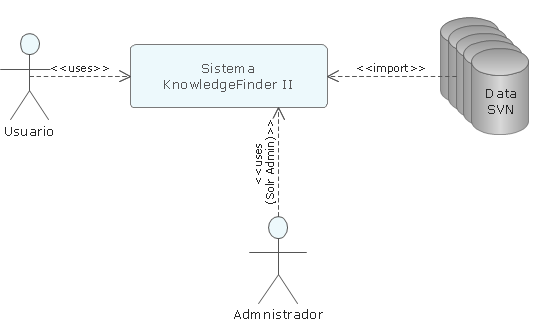
\includegraphics[width=0.8\textwidth]{Nivel0.png}
  \caption{Diagrama del ámbito y contexto de la arquitectura del sistema}
  \label{image:level0}
\end{figure}

\subsection{\IfLanguageName{english}{Hardware Architecture}{Arquitectura
Física}}

% En este apartado, describimos los principales elementos hardware que forman la arquitectura física de nuestro sistema, recogiendo por un lado los componentes del entorno de producción y los componentes de cliente.\\

% Se debe incluir un modelo de despliegue en el cual se describe cómo los elementos software son desplegados en los elementos hardware. También se incluyen las especificaciones y los requisitos del hardware (servidores, etc.), así como de los elementos software (sistemas operativos, servicios, aplicaciones, etc.) necesarios.
A continuación se va a describir el sistema de \gls{hardware} necesario que conforman la arquitectura física de nuestro sistema. En la figura \ref{image:deploview} podemos diferenciar los siguientes componentes:

\begin{itemize}

	\sitem{Cliente}
    Representa el \gls{hardware} que utiliza el usuario para acceder a los serivicios ofrecidos por \gls{kf2}. Éstos están dispolibles para ser usados por un navegador web o por un \gls{software} que permita el acceso a \glspl{sw}.
    
  	\sitem{Servidor para \gls{liferay} (\gls{tomcat})}
    Para alojar la instancia de \gls{liferay} que contendrá el \gls{sw} y el \gls{portlet} para la web de \gls{kf2} es necesario el \gls{hardware} apropiado para contener un servidor de \gls{tomcat}.
    
  \sitem{Servidor para \gls{solr}}
  El \gls{motorbusqueda} \gls{solr} puede estar instalado en varios tipos de servidores (\gls{tomcat}, \gls{jetty}, \dots). Para ello se requiere \gls{hardware} que pueda proporcionar alguno de estos. \Gls{solr} puede residir, por ejemplo, en la misma instancia de \gls{tomcat} donde se encuentra \gls{liferay} en ejecución.\\
  
  Este servidor debe tener acceso a los repositorios remotos o a una copia de trabajo local de \gls{svn} para el proceso de importación de los datos.
  
  \sitem{Control de acceso (nota)}
  Como medida de seguridad, se recomienda proteger el acceso a la instancia de \gls{solr} \cite{solrsecurity}. Para ello se pueden disponer de varias medidas de seguridad, por ejemplo un \gls{firewall}.
\end{itemize}

\begin{figure}[H]
  \centering
     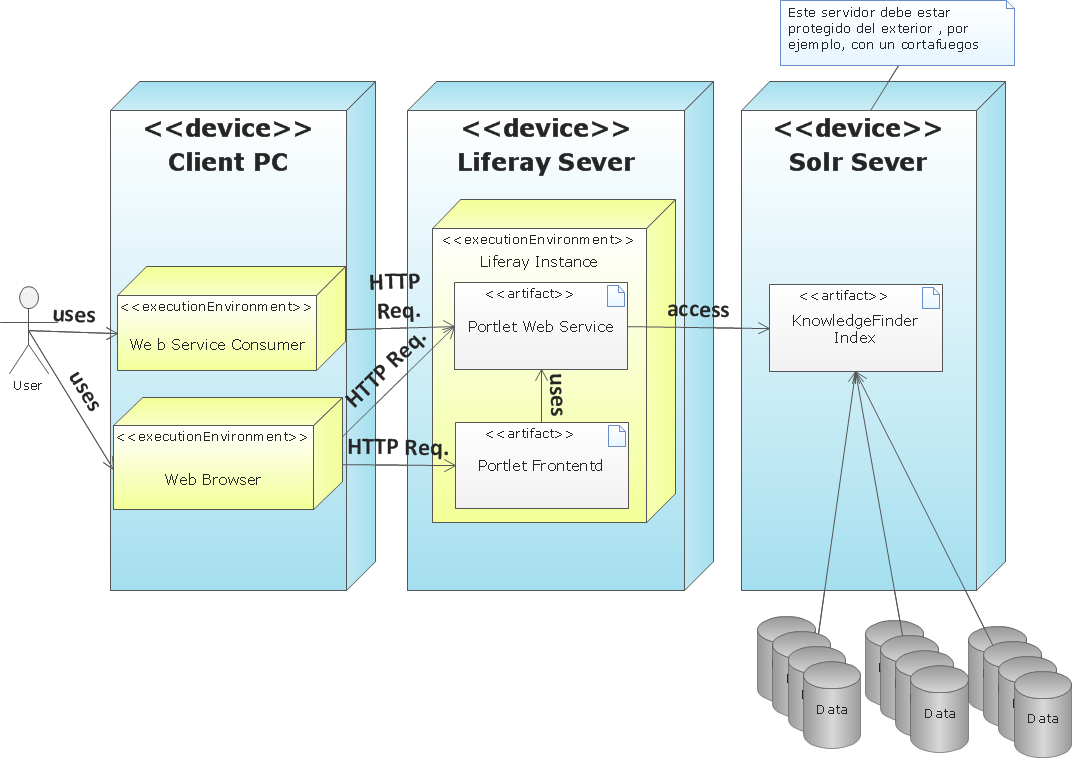
\includegraphics[width=\textwidth]{Despliegue.png}
  \caption{Diagrama de \gls{despliegue} para el proyecto \gls{kf2}}
  \label{image:deploview}
\end{figure}

\subsection{\IfLanguageName{english}{Software Architecture}{Arquitectura Lógica}} 

La arquitectura de diseño especifica la forma en que los artefactos software interactúan entre sí para lograr el comportamiento deseado en el sistema. En esta sección se muestra la comunicación entre el software base seleccionado, los componentes reutilizados y los componentes desarrollados para cumplir los requisitos de la aplicación. También se recogen los servicios de sistemas externos con los que interactúa nuestro sistema.\\

%Se debe incluir un diagrama de componentes que muestre en un alto nivel de abstracción los artefactos que conforman el sistema.\\

\subsection{Modelo Vista Controlador en \kfII}
Como se expuso en en apartado \ref{subsubsection:mvc}, el proyecto \gls{kf2} sigue una arquitectura de \gls{software} basada en el \gls{mvc}. A continuación se detalla cómo es el diseño aplicando esta arquitectura.



\begin{itemize}
	\sitem{El Modelo}
    En el caso de \gls{kf2} sería principalmente el índice de búsqueda. La información está almacenada en éste y es accesible gracias a la \gls{api} que proporciona el \gls{motorbusqueda}. 
    
    \sitem{El Controlador}
    El intermediario entre la vista y el índice de búsqueda es un 
\gls{sw} alojado en \gls{liferay}. De esta forma, el controlador tiene acceso a los roles del usuario definidos en \gls{liferay} que actualmente está usando la aplicación para definir su comportamiento. La respuesta del \gls{sw} variará para distintas combinaciones de roles de usuarios.
    
    \sitem{La Vista}
    Para el proyecto \gls{kf2} la vista representaría la página web donde se aloja la visualización y todos sus componentes. Es el interfaz principal del usuario para interactuar con el sistema.
\end{itemize}


\subsection{Desglose de Componentes}
\label{section:blocks}

Basándonos en el esquema expuesto en \cite{arc42} vamos a describir el la arquitectura del \gls{software} de \gls{kf2} por vistas de construcción. Comenzando por un nivel de abstracción donde se muestran los artefactos que conforman el sistema, se desglosará cada uno de ellos en sus componentes internas.\\

\subsubsection{Nivel 1 - Building View}
En la imagen \ref{image:level1} se puede ver como interactúa las distintos componentes del sistema \gls{kf2}. En ella también se aprecian las interfaces externas y los tres subsistemas principales que serán descritos en el siguiente nivel.
\begin{itemize}
	\sitem{Panel de administración de \gls{solr}} Interfaz para activar la importación de los datos.
    \sitem{Repositorios \gls{svn}} Conjunto de repositorios \gls{svn} desde donde se obtienen los datos.
    \sitem{Navegador de cliente} El usuario final interacciona directamente con el sistema usando un navegador web.
\end{itemize}

\begin{figure}[H]
  \centering
     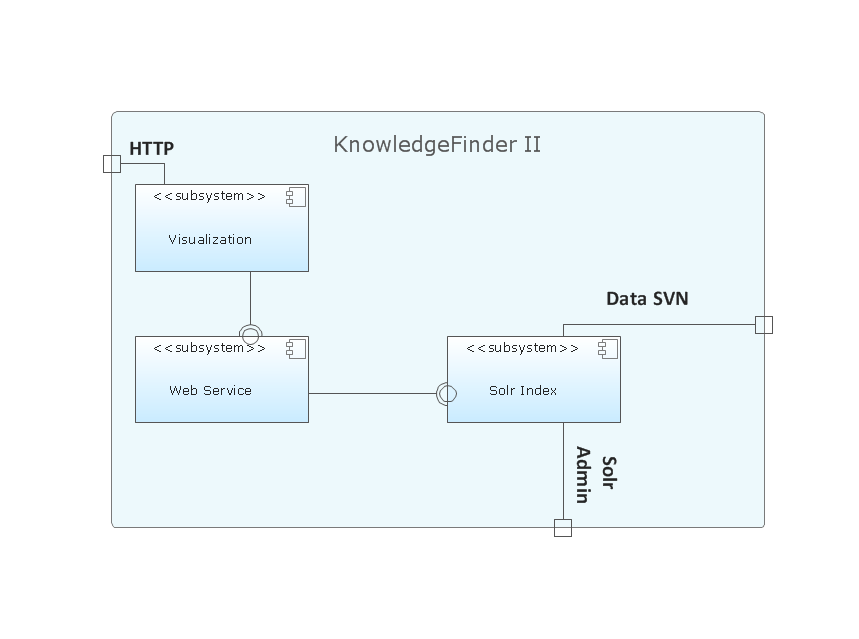
\includegraphics[width=\textwidth]{Nivel1.png}
  \caption{Nivel 1 - Building View \gls{kf2}}
  \label{image:level1}
\end{figure}


\subsubsection{Nivel 2 - Building View}
\label{subsubsection:n2building}
\sparagraph{Índice de búsqueda en \gls{solr}}
Este subsistema es responsable de la importación de la información para el índice de búsqueda de \gls{solr} desde los repositorios \gls{svn}. También se encarga de proporcionar estos datos importados a través de una \gls{api}. \\

Este subsistema de descompone los siguientes elementos representados en la imagen \ref{image:level2-solr}:
\begin{itemize}
	\sitem{\gls{svn} Crawler}
    Componente encargado de extraer los ficheros de \gls{svn} junto con todas sus propiedades. Recorre todo el repositorio (local o remoto) y empaqueta todas los elementos del repositorio.
    \sitem{\gls{svn} DataPicker}
    Componente encargado de transformar las extraer las propiedades de los elementos proporcionados por el crawler y empaquetarlos en objetos iterables de \gls{java}.
    \sitem{\gls{svn} Parser}
	Extrae las propiedades del \gls{svn} en formato \gls{json} y las prepara para la importación.
    \sitem{\gls{svn} DataImport}
    Se encarga de configurar y coordinar el proceso de importación.
    \sitem{\gls{solr} Tranformers}
    Transforma los datos durante la importación para adaptarlo a los requisitos específicos del índice.
    \sitem{\Gls{solr}}
    Instancia de \gls{solr} donde reside el índice importado. Proporciona la interfaz para importar y consultar los datos a través de una \gls{api} y un \gls{ui} web para su administración.
\end{itemize}

\begin{figure}[H]
  \centering
     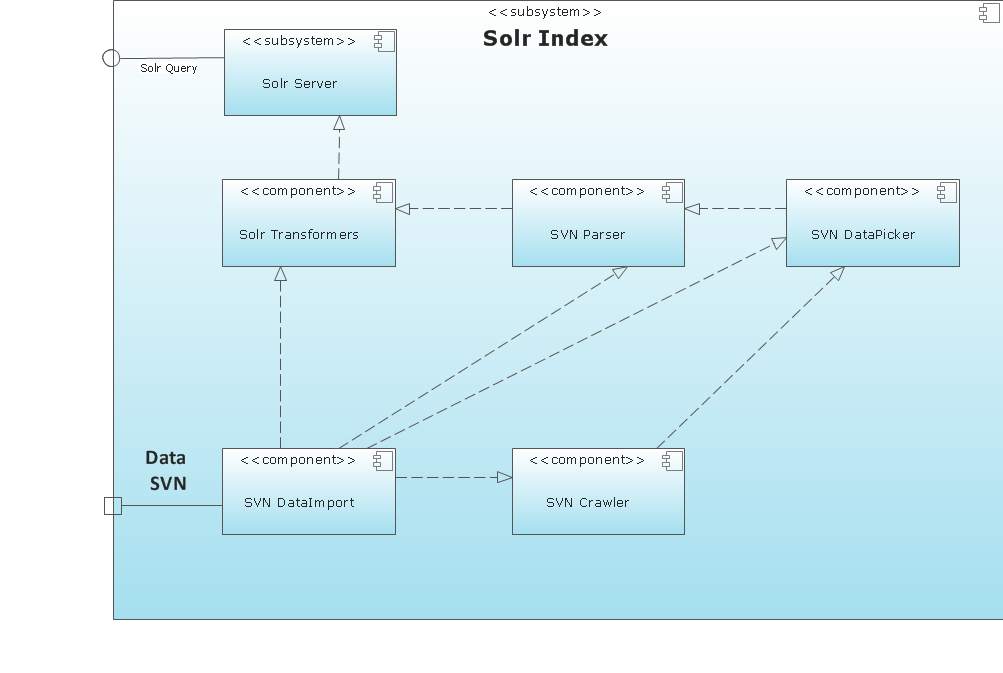
\includegraphics[width=\textwidth]{Nivel2Index.png}
  \caption{Nivel 2 - Building View Índice \gls{solr}}
  \label{image:level2-solr}
\end{figure}


\sparagraph{\Gls{sw}}
Este subsistema provee un \gls{sw} que permite acceder a los datos proporcionados por el índice de búsqueda \gls{solr}. Como muestra la imagen \ref{image:level2-sw}, se descompone en los siguientes elementos:
\begin{itemize}
	\sitem{KnowedgeFinder Service}
    Encargado de recibir las peticiones del \gls{sw} (get-document, get-nodes) y adaptar sus parámetros a la \gls{api} de \gls{solr}. Como resultado de las peticiones, crea una respuesta en formato \gls{json} con los valores pertinentes.
    \sitem{User-Query Factory}
    Elemento encargado de transformar las peticiones a la \gls{api} de \gls{solr} en función de los roles del usuario actual. 
\end{itemize}

\begin{figure}[H]
  \centering
     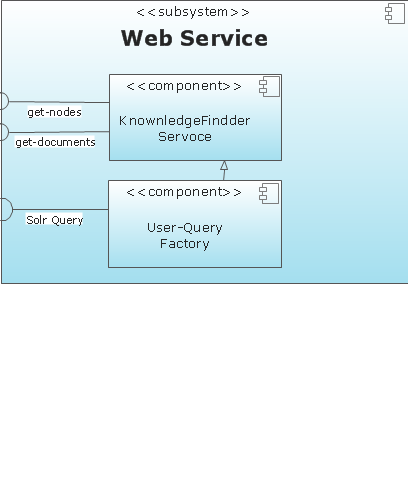
\includegraphics[width=0.5\textwidth]{Nivel2Webservice.png}
  \caption{Nivel 2 - Building View \Gls{sw}}
  \label{image:level2-sw}
\end{figure}

\sparagraph{Visualización}
El subsistema de visualización se encarga de proporcionar la \gls{ui} a través de elementos gráficos. A grandes rasgos, muestra la información obtenida a través del \gls{sw} de forma intuitiva y atractiva para el usuario. En la imagen \ref{image:level2-visual} se encuentran reflejados sus componentes y las relaciones entre ellos:

\begin{itemize}
	\sitem{TemplateController}
    Controlador que genera una página de \gls{jsp} para una \gls{url} definida por el administrador. 
    
    \sitem{Filters Loader}
    Este componente crea los filtros necesarios a partir de los \glspl{metadato} obtenido en peticiones al \gls{sw}.
    
    \sitem{Página \gls{html}}
    La página \gls{jsp} obtiene la información del TemplateController genera una página \gls{html}. Con los Filters Loader crea variables que son necesarias por todos los componentes \gls{js}.
    \sitem{Main.js}
    Encargado de cargar todos los componentes de \gls{js}. También coordina los evento del usuario y el comportamiento de los componentes entre ellos.
  	\sitem{d3.knowledgefinder.graph.js}  
    Componente encargado de crear un grafo que representa los \glspl{metadato} y las relaciones entre ellos.
    \sitem{d3.knowledgefinder.modal.js}
    Componente que genera una ventana emergente con los detalles de un documento previamente seleccionado de la lista de resultados.
    \sitem{d3.knowledgefinder.result.js}
	Lista los documentos obtenidos durante la consulta y los organiza usando un sistema de \gls{paginacion}.
    \sitem{d3.knowledgefinder.selection.js}
    Componente encargado de mostrar una lista de botones con los actuales parámetros de búsqueda. A través de esta lista el usuario puede consultar y desactivar los elementos que componen la búsqueda.
    \sitem{d3.knowledgefinder.table.js}
    La tabla generada por el componente de Página \gls{html} es manipulada a través de este componente de acuerdo a los resultados y búsquedas.
    \sitem{d3.knowledgefinder.urlquery.js}
    Componente auxiliar para manipular los parámetros y facilitar al resto de componentes de la visualización la comunicación con el \gls{sw}. 
\end{itemize}
\begin{figure}[H]
  \centering
     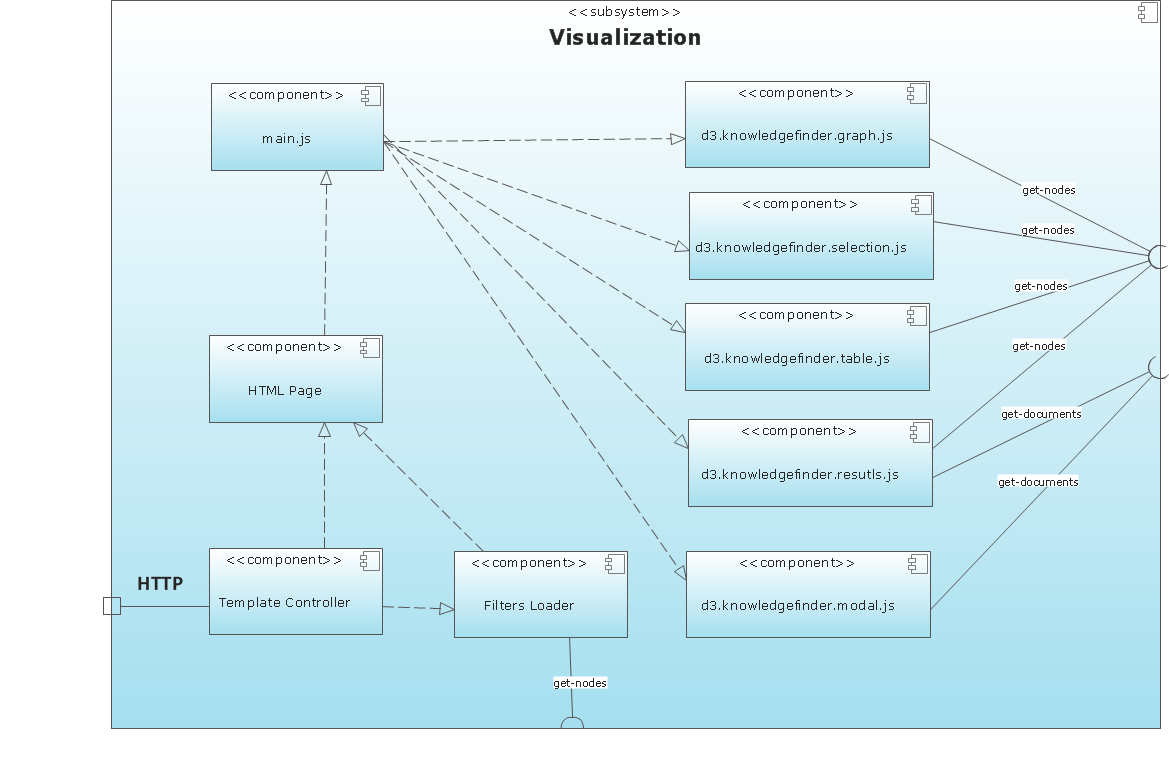
\includegraphics[width=\textwidth]{Nivel2Visualization.png}
  \caption{Nivel 2 - Building View Visualización}
  \label{image:level2-visual}
\end{figure}

%Existen diferentes patrones o estilos arquitectónicos. En los sistemas web de información es común la utilización del patrón Layers (Capas), con el cual estructuramos el sistema en un número apropiado de capas, de forma que todos los componentes de una misma capa trabajan en el mismo nivel de abstracción y los servicios proporcionados por la capa superior utilizan internamente los servicios proporcionados por la capa inmediatamente inferior. Habitualmente se tienen las siguientes capas:

\begin{comment}
\paragraph*{\IfLanguageName{english}{Presentation Tier (frontend)}{Capa de
presentación (frontend)}} Este grupo de artefactos software conforman la capa de presentación del sistema, incluyendo tanto los componentes de la vista como los elementos de control de la misma.

\paragraph*{\IfLanguageName{english}{Application Tier}{Capa de negocio}}
Este grupo de artefactos software conforman la capa de negocio del sistema, incluyendo los elementos del modelo de dominio y los servicios (operaciones del sistema).

\paragraph*{\IfLanguageName{english}{Data Tier}{Capa de persistencia}}
Este grupo de artefactos software conforman la capa de integración del sistema, incluyendo las clases de abstracción para el acceso a datos (BD o sistema de ficheros) o a sistemas heredados.\\

Es común que a la capa de negocio y de datos de los sistemas web, se denomine conjuntamente como backend o modelo de la aplicación.

Opcionalmente, podemos disponer de un conjunto de artefactos software que pueden ser usados por elementos de cualquiera de las capas del sistema y que fundamentalmente proporcionan servicios relacionados con requisitos no funcionales (calidad).
\end{comment}

\begin{comment}
\section{\IfLanguageName{english}{Parameterization of the Based
Software}{Parametrización del software base}} 
\question{Tengo que poner algo en mi caso aquí????}
\todo[inline]{En esta sección, se detallan las
modificaciones a realizar sobre el software base, que son requeridas para la correcta construcción del sistema. En esta sección incluiremos las  actuaciones necesarias sobre la interfaz de administración del sistema, sobre el código fuente o sobre el modelo de datos.}
\end{comment}

\section{\IfLanguageName{english}{Physical Data Design}{Diseño Físico de Datos}}
\begin{comment}
En esta sección se define la estructura física de datos que utilizará el sistema, a partir del modelo de conceptual de clases, de manera que teniendo presente los requisitos establecidos para el sistema de información y las particularidades del entorno tecnológico, se consiga un acceso eficiente de los datos.
La estructura física se compone de tablas, índices, procedimientos almacenados, secuencias y otros elementos dependientes del SGBD a utilizar.
\end{comment}
La estructura física de los datos que utiliza el sistema es el índice de búsqueda de \gls{solr}. Su definición se describe en el esquema. Estos esquemas deben definirse dependiendo de las necesidades de cada instancia del \gls{framework} \gls{kf2}.\\

A continuación se detalla en la tabla \ref{table:index} en detalle la estructura del índice de búsqueda una vez que la importación ha finalizado (instancia del proyecto \gls{strada} de \gls{kf2}). En ella se puede observar, entre otros datos, qué campos se utilizan para la búsqueda \gls{fulltext}, los campos que son creados en el momento de la importación (dinámicos), qué campos son usados para la búsqueda en el índice, etcétera .

\begin{center}
\begin {table}[H]
    \begin{tabular}{| l | c | l | c | c | c | p{5cm} |}
    \hline
    \rot{\textbf{Campo}} & \rot{\textbf{Obligatorio}} & \rot{\textbf{Tipo}} & \rot{\textbf{Múltiple}} & \rot{\textbf{Index}} & \rot{\textbf{Stored}} & \rot{\textbf{Notas}}		\\ \hline
    id  			& X & string 		&   & X & X	& Unique Key  	 	\\ \hline
    title 			& X & text			&   & X & X & \Gls{fulltext}    \\ \hline
    description     &   & text    	 	&	&  	& X	& \Gls{fulltext}    \\ \hline
    keywords 		&   & string 		& X & X & X	& \Gls{fulltext}    \\ \hline
    categories      &  	& string 		& X &  	& X	& 					\\ \hline
    filePath 		& 	& string 		& 	&   & X	&				\\ \hline
    institute 		&   & string 		& 	&   & X & Generado durante la importación \\ \hline
 timePeriodOfDataCollection &  & string &   &   & X	&				\\ \hline
 startTimePeriodOfDataCollection &  & date &   & X & X	&				\\ \hline
 endTimePeriodOfDataCollection &  & date &   & X & X	&				\\ \hline
 startDateDate		 &  & date 			&   & X & X	&				\\ \hline
 temporalCoverage    &  & string 		&   &  	& X	& 					\\ \hline
 startTemporalCoverage &  & date &   & X & X	&				\\ \hline
 endTemporalCoverage &  & date &   & X & X	&				\\ \hline
 spatialCoverage &  & string & X &   & X	&				\\ \hline
 world &  & string & X & X  & 	& Generado desde spatialCoverage \\ \hline
 regionsWorld &  & string & X & X  & 	& Generado desde spatialCoverage \\ \hline
 countries &  & string & X & X  & 	& Generado desde spatialCoverage \\ \hline
 regions &  & string & X & X  & 	& Generado desde spatialCoverage \\ \hline
 size\_author & & int & & & X & Generado desde authors \\ \hline
 contentcreationdatetime & & int & & X &  & Propiedad interna de \gls{svn} \\ \hline
 contentmodificationdatetime & & int & & X &  & Propiedad interna de \gls{svn} \\ \hline
 author\_uid\_* & & string & & & X & Generado desde authors (campo dinámico), \Gls{fulltext} \\ \hline
 author\_firstName\_* & & string & & & X & Generado desde authors (campo dinámico), \Gls{fulltext} \\ \hline
 author\_lastName\_* & & string & & & X & Generado desde authors (campo dinámico), \Gls{fulltext} \\ \hline
 author\_mail\_* & & string & & & X & Generado desde authors (campo dinámico), \Gls{fulltext} \\ \hline
 author\_organization\_* & & string & & & X & Generado desde authors (campo dinámico), \Gls{fulltext} \\ \hline
  category\_* & & string & X & X & X & Generado desde categories (campo dinámico), \Gls{fulltext} \\ \hline
    \end{tabular}
    \caption{Tabla resumen del esquema de \gls{kf2} de \gls{solr} para el proyecto \gls{strada}}
    \label{table:index}
  \end{table}
\end{center}

\begin{comment}

% Reemplazado por la vista de procesos 
\section{\IfLanguageName{english}{Detailed Component Design}{Diseño detallado de Componentes}}
Para cada uno de los módulos funcionales del sistema debemos realizar un diagrama de secuencia, para definir la interacción existente entre las clases de objetos que permitan responder a eventos externos.
\end{comment}

\section{Vista de Procesos}
Siguiendo nuevamente el esquema expuesto  en \cite{arc42}, en esta sección se describe el comportamiento de los componentes del sistema descritos en la sección \ref{section:blocks} como elementos de ejecución.\\

A continuación se describen los escenarios más interesantes y los casos de uso más importantes del sistema destacando qué componentes de los subsistemas y qué subsistemas tienen mayor relevancia con mayor transcendencia para el lector de esta documentación.

\subsection{Iniciación de la Visualización}
La página web que contiene la visualización debe ser inicializada en el servidor cuando un usuario realiza una consulta sobre la \gls{url} correcta.\\

El primer paso lo realiza el controlador del \gls{portlet}. Éste adquiere los filtros y establece los elementos del menú a través de llamadas al \gls{sw}. Una vez que obtiene todos los datos, genera la página \gls{jsp}. Cuando la página ha sido creada se inicializan todos los componentes de \gls{js} usando nuevamente llamadas al \gls{sw}. Este proceso se describe con más detalles en la imagen \ref{image:runtime-init}.


\begin{figure}[H]
  \centering
  	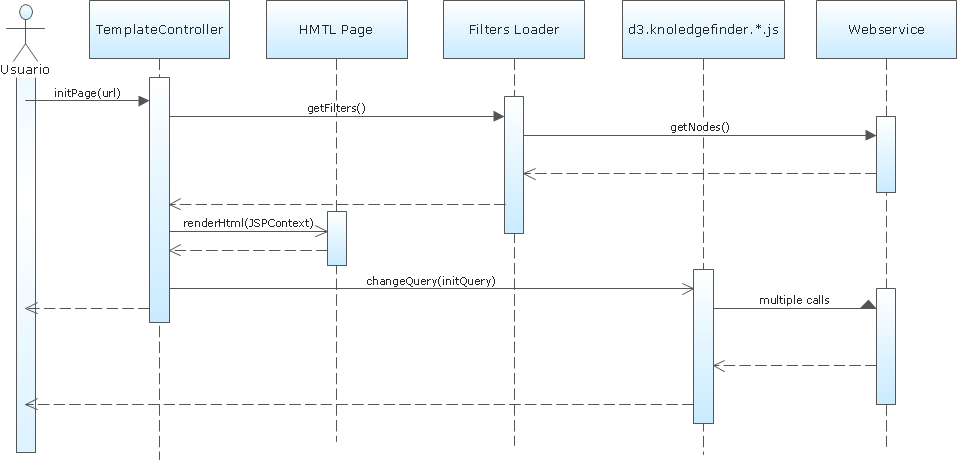
\includegraphics[width=\textwidth]{SE2init.png}
  \caption{Diagrama de Secuencia - Iniciación de la Visualización}
  \label{image:runtime-init}
\end{figure}

\subsection{Ejecución de Consulta}
Cuando el usuario ejecuta una consulta añadiendo o eliminando algún filtro, por ejemplo, seleccionando un elemento del menú o introduciendo un valor en el campo \gls{fulltext} el sistema debe obtener el nuevo estado para todos los componentes de la \gls{ui}.\\

Concretamente, la lista de resultados debe mostrar el nuevo conjunto de documentos fruto de la nueva consulta. El grafo debe calcular los nuevos valores para sus componentes y redibujarlos en función de éstos. El menú debe adecuarse igualmente al nuevo estado de la aplicación. Para todo ello, se realizan diversas consultas al \gls{sw} de forma asíncrona adaptadas a cada componente. El gráfico representado en la imagen \ref{image:runtime-query} esquematiza este comportamiento.

\begin{figure}[H]
  \centering
  	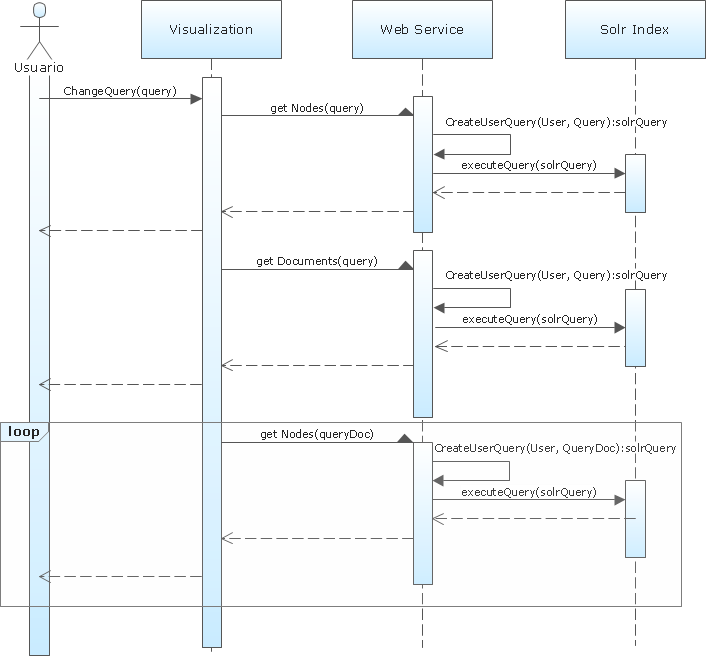
\includegraphics[width=1\textwidth]{SEChangeQ.png}
  \caption{Diagrama de Secuencia - Ejecución de Consulta}
  \label{image:runtime-query}
\end{figure}

\subsection{Modificación del Grafo de Exploración}
Sin modificar la consulta, el usuario puede modificar los grupos que se muestran en el grafo a través de las opciones del menú. El grafo obtiene los valores para este nuevo estado a través de consultas al \gls{sw}. Con el diagrama de secuencia de la imagen \ref{image:runtime-graph} se representa este proceso.

\begin{figure}[H]
  \centering
  	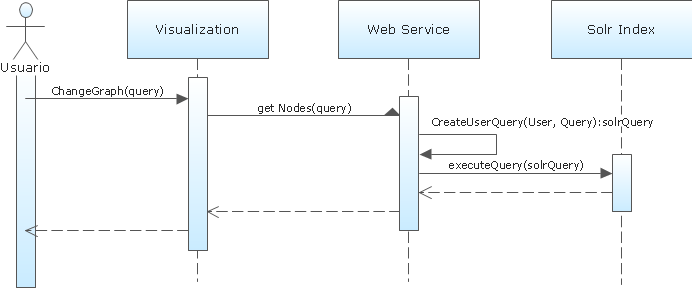
\includegraphics[width=1\textwidth]{SEChangeGraph.png}
  \caption{Diagrama de Secuencia - Modificación del Grafo de Exploración}
  \label{image:runtime-graph}
\end{figure}

\subsection{Modificación de la Lista de Resultados}
La lista de resultados está organizada en páginas y ordenada por según la elección del usuario dentro de unas posibles opciones. Tanto si el usuario cambia de página usando los elementos de la \gls{paginacion} o selecciona otro criterio de ordenación el sistema debe actualizar los elementos de esta lista a través de consultas al \gls{sw}. En la imagen \ref{image:runtime-results} se expone el diagrama de secuencia para estas acciones.

\begin{figure}[H]
  \centering
  	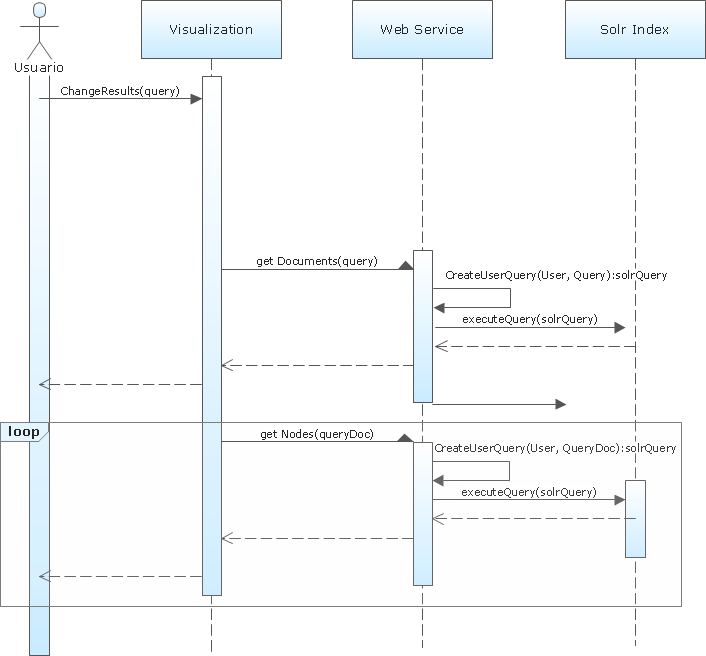
\includegraphics[width=1\textwidth]{SEChangeResults.png}
  \caption{Diagrama de Secuencia - Modificación de la Lista de Resultados}
  \label{image:runtime-results}
\end{figure}


\begin{comment}
Alternative terms:

Dynamic view
Process view
Workflow view
This view describes the behavior and interaction of the system’s building blocks as runtime elements (processes, tasks, activities, threads, …).

Select interesting runtime scenarios such as:

How are the most important use cases executed by the architectural building blocks?
Which instances of architectural building blocks are created at runtime and how are they started, controlled, and stopped.
How do the system’s components co-operate with external and pre-existing components?
How is the system started (covering e.g. required start scripts, dependencies on external systems, databases, communications systems, etc.)?
 

Note: The main criterion for the choice of possible scenarios (sequences, workflows) is their architectural relevancy. It is not important to describe a large number of scenarios. You should rather document a representative selection.

Candidates are:

1.The top 3 – 5 use cases

2.System startup

3.The system’s behavior on its most important external interfaces

4.The system’s behavior in the most important error situations

 

Motivation
Esp. for object-oriented architectures it is not sufficient to specify the building blocks with their interfaces, but also how instances of building blocks interact during runtime.

This view explains how the blocks interact, how they provide their functionality, how the systems works.

 

Form
Document the chosen scenarios using UML sequence diagrams, activity diagrams or communications diagrams. Enumerated lists are sometimes feasible.

Using object diagrams you can depict snapshots of existing runtime objects as well as instantiated relationships. The UML allows to distinguish between active and passive objects.
\end{comment}

\section{\IfLanguageName{english}{Detailed Design of the User Interface}{Diseño detallado de la Interfaz de Usuario}}
\begin{comment}
En esta sección se detallarán las interfaces entre el sistema y el usuario, incluyendo un prototipo de alta fidelidad con el diseño de la IU. Se definirá el comportamiento de las diferentes pantallas, indicando qué ocurre en los distintos componentes visuales de la interfaz cuando aparecen y qué acciones se disparan cuando el usuario trabaja con ellas.
\end{comment}
En esta sección se va a describir con detalle el diseño y el comportamiento de la \gls{ui} del \gls{framework} \gls{kf2}. Para esta versión se definen dos pantallas; la pantalla principal y la pantalla de detalles de documento.


\subsection{Pantalla Principal}
La pantalla principal de la aplicación se puede observar en la imagen \ref{image:uiprincipal}. Como la figura indica, se diferencian cinco componentes que a continuación se exponen.

\begin{figure}[h!]
  \centering
  	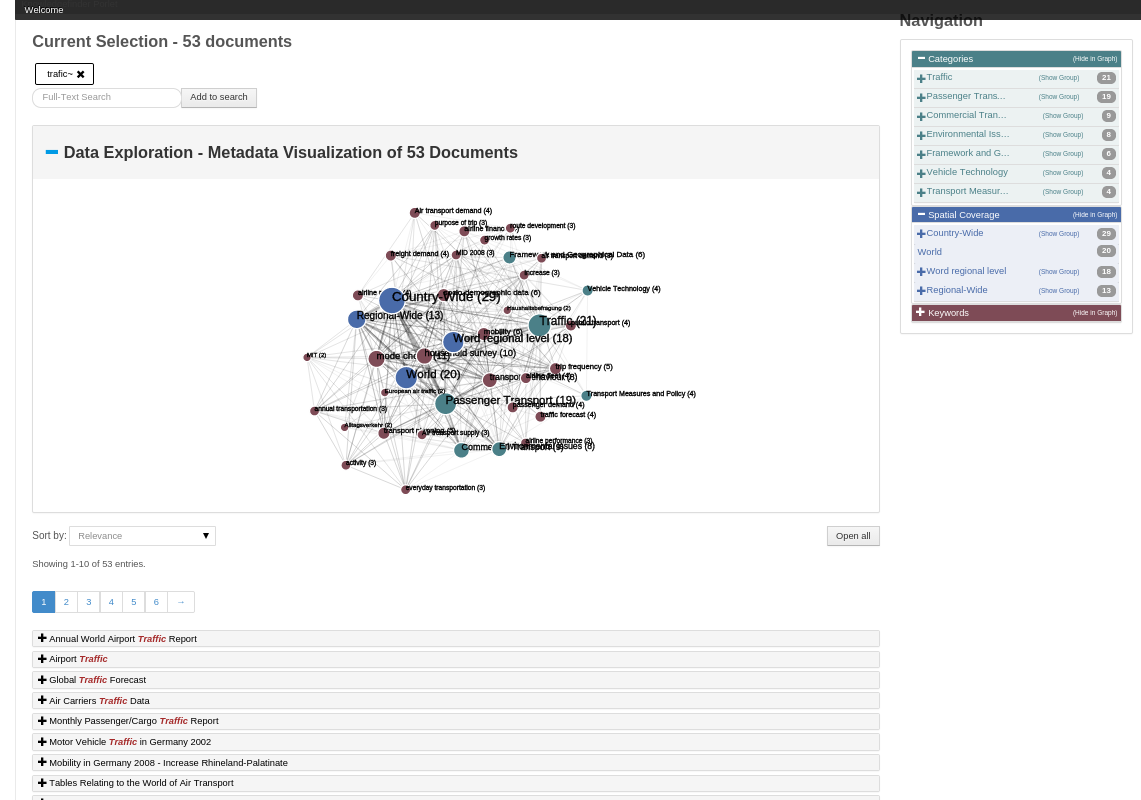
\includegraphics[width=1\textwidth]{general_ap.png}
  \caption{Pantalla principal}
  \label{image:uiprincipal}
\end{figure}

\subsubsection{Grapo de Exploración}
Representa el elemento más importante de la visualización. En el grafo se representa los filtros aplicables a los documentos que concuerdan con la búsqueda aplicada. Cada filtro representa un nodo y las aristas las relación entre nodos, el número de documentos con ambos filtros. El tamaño de los nodos y el grosor de las aristas está directamente relacionado con el número de documentos para cada elemento.\\

Cuando el usuario pulsa sobre algún nodo o alguna arista del grafo se aplican los correspondientes filtros.

\subsubsection{Menú}
Ofrece todos los posibles filtros de \glspl{metadato} disponibles. Están ordenados por números de documentos afectados por el filtro y se reordenan cuando estos valores cambian.\\

Se agrupan en, como máximo, dos subniveles siendo el elemento principal de cada grupo. Estos grupos se representan en modo acordeón con un posible \gls{scroll} sobre las listas de filtros.\\

A través de un botón en los encabezados de los grupos, el usuario podrá seleccionar qué grupos serán mostrados en el gráfico y pulsando sobre los elementos del menú, qué filtros se han de aplicar para búsqueda.
 
\subsubsection{Lista de Resultados}
Los resultado de la búsqueda realizada en cada momento es mostrada en una lista con los títulos de los documentos. Esta lista está dividida usando un sistema de \gls{paginacion}.\\

Cuando el usuario pulsa sobre algún elemento de la lista, se despliega una sección en forma de acordeón con la descripción del documento seleccionado y un botón para desplegar sus detalles en una ventana emergente (ver sección \ref{subsection:detalles}). También se puede desplegar/plegar este acordeón para todos los elementos de la lista pulsando un botón y  puede ser ordenada por varios criterios seleccionables a través de un menú \textit{Drop-down}.

\subsubsection{Filtros Aplicados}
En la parte superior de la pantalla principal se muestran los filtros actuales y cadenas de búsquedas aplicadas. Pulsando sobre ellos se eliminan de los criterios de búsqueda.

\subsubsection{Comportamientos Transversales}
Los componentes anteriormente descritos se relacionan entre sí a través de los siguientes cuando el usuario se posiciona en un elemento del grafo o sobre uno del menú:
    \begin{itemize}
    	\item El grafo muestra resaltado respecto al resto de elementos el subgrafo compuesto por las componentes conexas del filtro en cuestión.
   		\item En el menú de elementos se resalta el filtro.
   		\item En la lista de resultados se resaltan los que tienen relación ese filtro.
   \end{itemize}

\subsubsection{Campo \gls{fulltext}}
Entre el grafo de exploración y los filtros aplicados  se encuentra un simple formulario para la introducción de cadenas de búsqueda. En ella, el usuario puede de definir su propias cadenas de búsqueda.

\subsection{Pantalla de Detalles de Documento}
\label{subsection:detalles}
Como se ha explicado antes, los detalles de los documentos se exponen en una ventana emergente. En la imagen \ref{image:uidetalles} se observa la simpleza de ésta. Se muestran los campos configurados para cada usuario y la opción de cerrar la ventana para volver a la pantalla anterior.

\begin{figure}[h!]
  \centering
  	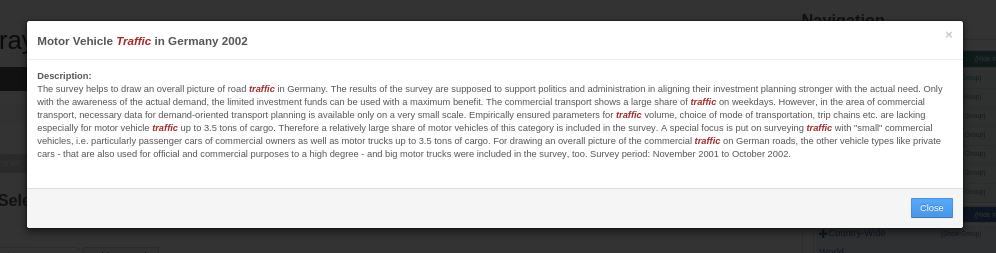
\includegraphics[width=1\textwidth]{hightpopp.png}
  \caption{Pantalla detalles de documento}
  \label{image:uidetalles}
\end{figure}


